%% Results text for the 2023--2025 window. Numbers from code/results/bench (200 portfolios, 100 for ablations).
\subsection{\blt{Results on the 2023--2025 Test Period}} \label{s:results}
Table~\ref{tab:bench_mean} reports the means over the 200 portfolios, Table~\ref{tab:bench_paired} the paired tests, Fig.~\ref{fig:bench_wealth} the median wealth paths and Fig.~\ref{fig:bench_sharpe} the distribution of the annualised Sharpe ratio.

\emph{The constrained-QP policy.} With the corrected optimiser the Risk-Averse policy (RA) has an annualised Sharpe ratio of $0.34$ and a total return of $1.11$, against $0.66$ and $1.27$ for the daily rebalanced equal-weight portfolio and $0.77$ and $1.36$ for equal-weight buy and hold. The differences are significant on every portfolio-level test (Wilcoxon $p<0.001$, RA better in 26\% and 20\% of the portfolios, respectively). The cause is visible in the last two columns: RA trades $15\%$ of the portfolio value per day and pays $15\%$ of the initial wealth in transaction costs over the two years, ten times more than the rebalanced equal-weight portfolio. Its gross performance (before costs) is comparable to the equal-weight benchmarks; it is the turnover that is not. RA does deliver what its name promises on one axis: its maximum drawdown ($-25.5\%$) is smaller than that of both equal-weight portfolios and much smaller than that of every mean-variance variant ($-40\%$ to $-42\%$), and its volatility is the lowest of the non-min-variance strategies. The only min-variance portfolio it does not beat on drawdown uses a 250-day window.

\emph{Why the turnover is high.} The risk weight $\omega^*$ of Sec.~\ref{s:FPD} is the minimiser of \eqref{e:idealbehaviourminomega} over $\omega>0$; in every one of the $10^5$ decision steps of the experiment the result is the upper bound of the search interval, $\omega_{\max}=10^3$. The necessary condition for an extreme stated in Sec.~\ref{s:FPD} is a sum of two terms that are positive for $\mat{D}\succ0$, $\hat{\mat{\Sigma}}\succeq0$ and $\omega>0$, so it has no root; the implementation minimises its left-hand side, which decreases monotonically in $\omega$, and the elicitation reduces to ``as risk-averse as allowed''. Sec.~\ref{s:sensitivity} treats $\omega_{\max}$ as the user-set quantity it effectively is. With $\omega=10^3$ the variance term $\tfrac{1}{2}\omega^2 a^\top\hat{\mat{\Sigma}}a$ in \eqref{e:lossmatrixQdefinition} is four orders of magnitude larger than the transaction-cost term $(a_t-a_{t-1})^\top\mat{D}(a_t-a_{t-1})$, so the cost is effectively not in the loss, and the policy re-optimises the minimum-variance-like allocation from scratch every day on a covariance estimate that is itself updated with heavy forgetting (Sec.~\ref{s:ablation_results}). The sensitivity study in Sec.~\ref{s:sensitivity} caps $\omega_{\max}$ and confirms this reading. This is also the mechanism behind the small drawdowns.

\emph{The legacy (softmax) policy.} The policy that produced the tables of the earlier version of this paper keeps the weights within a few percent of uniform (mean daily turnover $2.9\%$). Under the common cost model it is statistically indistinguishable from the rebalanced equal-weight portfolio in return and loses to it slightly but consistently in Sharpe ratio ($-0.03$, $p<0.001$, better in 1\% of the portfolios); it beats the min-variance and 120-day mean-variance portfolios in Sharpe ratio and all mean-variance portfolios in drawdown. Our earlier claim of outperforming the uniform portfolio rested on charging the uniform portfolio no costs and on the heuristic's near-uniform weights; it does not survive a paired test with identical cost treatment.

\emph{Classical benchmarks.} Plain mean-variance on a 250-day window has the highest return among the stock-universe strategies ($1.57$) at the price of a $-40\%$ maximum drawdown and a $37\%$ annualised volatility; its cost-aware variant halves the turnover of the 120-day version without changing the picture. The ARX-conditional mean-variance, which feeds the same regressors selected by our structure estimation into a ridge regression and a Markowitz optimiser with the same risk aversion $\omega^*$, loses money ($0.73$): the point forecasts of daily returns from these regressors are not tradeable through a classical optimiser, and the Bayesian learning with the FPD loss is what keeps RA from doing the same (RA beats it in $99.5\%$ of the portfolios). The S\&P~500 over the same days returned $1.62$ with a Sharpe ratio of $1.58$ and a drawdown of $-19\%$; no strategy on this 20-stock universe approaches it, including equal-weight buy and hold, which says more about the universe selected by the 2021 screen than about any allocation rule. We therefore do not claim to beat the index.

\begin{figure}[ht!]\centering
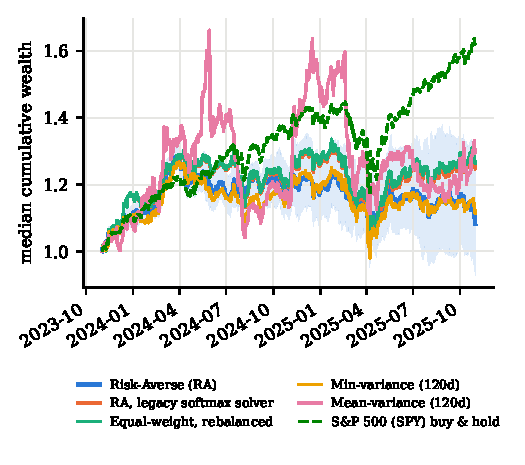
\includegraphics[width=0.48\textwidth]{Images/bench_wealth.pdf}
\caption{Median cumulative wealth over the 200 portfolios (band: interquartile range of RA). S\&P~500 is the same for all portfolios.}
\label{fig:bench_wealth}
\end{figure}
\begin{figure}[ht!]\centering
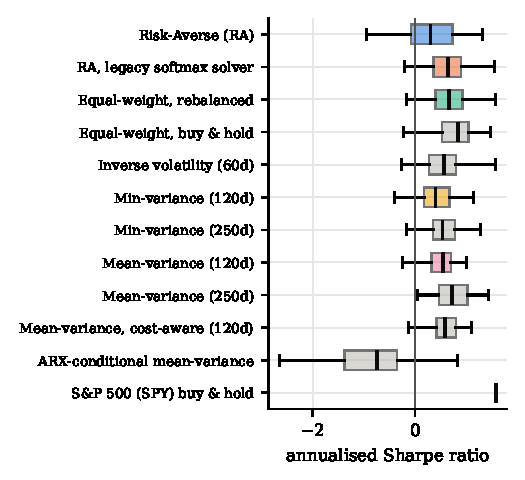
\includegraphics[width=0.48\textwidth]{Images/bench_sharpe.pdf}
\caption{Annualised Sharpe ratio across the 200 portfolios (boxes: quartiles, whiskers: 1.5 IQR).}
\label{fig:bench_sharpe}
\end{figure}

\subsection{\blt{Ablation Study}} \label{s:ablation_results}
Table~\ref{tab:ablation} and Fig.~\ref{fig:bench_ablation} isolate the components on 100 portfolios.
\begin{itemize}\setlength{\itemsep}{1pt}
\item \emph{Optimiser.} The corrected SMALBE of Sec.~\ref{s:optimization} and the SLSQP reference give identical allocations (maximum weight difference $3\cdot10^{-7}$), so the results do not depend on the QP solver; the softmax heuristic is a different policy (Sec.~\ref{s:results}).
\item \emph{Risk term.} Removing the FPD risk term (risk-neutral quadratic loss) is catastrophic: the policy chases the point forecast, turns the portfolio over $1.5$ times per day and loses $72\%$. The same happens with Thompson sampling of $\theta$ in the design ($-56\%$) and without structure estimation ($-49\%$): the parameter uncertainty of a 137-regressor model, or a sampled parameter, produces forecasts that the loss then trusts. The FPD risk term, the structure estimation and the point estimate are what make the daily return forecasts usable at all.
\item \emph{Forgetting.} Replacing the data-based forgetting by a plain Bayesian update changes nothing measurable (Sharpe $+0.04$, $p=0.13$); exponential forgetting $0.99$ is worse ($-0.22$, $p<0.001$). The median weights in Fig.~\ref{fig:bench_forgetting} explain why: the optimiser keeps $\gamma$, the weight of the prior, between $0.5$ and $0.8$ on almost every day, so the statistic is pulled more than half-way back to $\mat{V}_0$ daily and the model never moves far from the prior fitted on the first 125 days. The mechanism the forgetting was designed for is visible at the April 2025 tariff shock (shaded), where $\beta$ drops to zero and $\gamma$ rises, i.e.\ the outlying days are discarded; but on ordinary days the same mechanism discards most of the data as well.
\item \emph{Prior.} The flat prior gives the best numbers of all RA variants (Sharpe $0.72$, total return $1.30$, turnover $1.6\%$), but for a trivial reason: its allocations coincide with the rebalanced equal-weight portfolio to three decimals in every metric. With $\mat{V}_0=10^{-6}\mat{I}$ the forgetting pulls the statistic back to an isotropic covariance and to zero forecasts every day, and the constrained minimiser of a quadratic loss with $\hat{\mat{\Sigma}}\propto\mat{I}$ and $\hat y=0$ is $1/N$. The optimal prior of Sec.~\ref{s:prior} with $\mu=0.9$ is worth $\mu/(1-\mu)=9$ times the 125 days it is built from, i.e.\ 1125 days of pseudo-data; the sensitivity study (Sec.~\ref{s:sensitivity}) shows that $\mu=0.7$, which keeps fewer regressors and a weaker prior, is better than $0.9$, and that the forgetting prior $(\alpha_0,\beta_0)$ changes the forgetting weights but not the result.
\item \emph{Horizon.} The receding horizon $h=5$ without loss-to-go propagation gives the same allocations as $h=1$ with propagation (maximum weight difference $7\cdot10^{-6}$). At $\omega=10^3$ the one-step quadratic loss dominates the loss-to-go by orders of magnitude and the multi-step design is inactive.
\end{itemize}
\begin{figure}[ht!]\centering
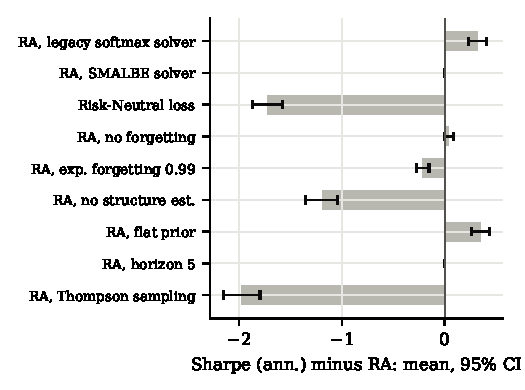
\includegraphics[width=0.48\textwidth]{Images/bench_ablation.pdf}
\caption{Annualised Sharpe ratio of each ablation minus that of the full Risk-Averse policy, paired over 100 portfolios (mean and bootstrap 95\% CI).}
\label{fig:bench_ablation}
\end{figure}
\begin{figure}[ht!]\centering
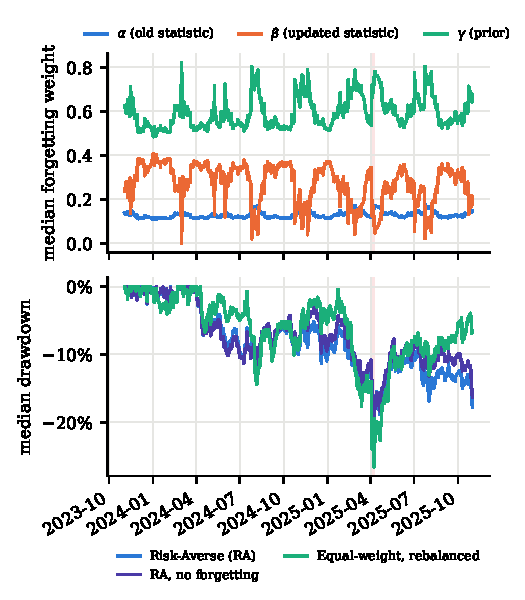
\includegraphics[width=0.48\textwidth]{Images/bench_forgetting.pdf}
\caption{Top: median optimal forgetting weights over the 200 portfolios. Bottom: median drawdown of RA, RA without forgetting and the rebalanced equal-weight portfolio; shaded: the tariff shock of 2--9 April 2025.}
\label{fig:bench_forgetting}
\end{figure}

\subsection{\blt{Stress Tests: Outliers and Parameter Changes}} \label{s:stress}
Fig.~\ref{fig:stress_synthetic} uses ARX data with known parameters (4 assets, 6 regressors, 700 days), two one-day crashes of $-12\%$ on all assets (days 300 and 450) and a sign flip of all regression coefficients at day 550. Three learners see identical data and start from the same optimal prior. On the crash days the data-based forgetting sets $\beta=0$ and $\gamma\approx1$: the outlier is discarded and the statistic reverts to the prior, and the estimation error does not move, whereas both other learners absorb the outlier (visible as a jump of the error after day 300 for the no-forgetting learner). This is the robustness to black-swan observations claimed in Sec.~\ref{s:forgetting}, and it holds. The same figure shows the price: during the stationary phase the optimal forgetting keeps the estimation error at its prior level ($0.72$) while the other learners improve to $0.5$, and after the parameter change it does not re-learn (the weights return immediately to their prior values, $\gamma\approx0.43$) while exponential forgetting halves the error within 150 days. Table~\ref{tab:ablation} showed the corresponding market result: no forgetting is at least as good. In its present form the mechanism therefore protects against outliers but not against slow or abrupt drift, and it does so by not learning; a forgetting prior $(\alpha_0,\beta_0,\gamma_0)$ that places less mass on $\gamma$ (Sec.~\ref{s:sensitivity}) is the obvious knob.
\begin{figure}[ht!]\centering
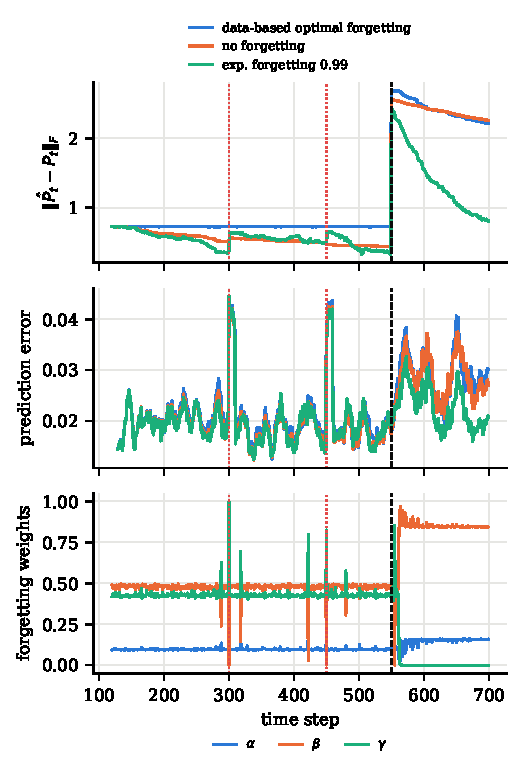
\includegraphics[width=0.48\textwidth]{Images/stress_synthetic.pdf}
\caption{Synthetic stress test. Top: parameter estimation error; middle: one-step prediction error (10-day mean); bottom: the optimal forgetting weights. Dotted: one-day crashes; dashed: change of all regression coefficients.}
\label{fig:stress_synthetic}
\end{figure}

